%PIP-412035RC020
\documentclass[reprint,amsmath,amssymb,aps,prb,footinbib,floatfix]{revtex4-2}
\bibliographystyle{apsrev4-2}
\usepackage{afterpage}
\usepackage{blindtext}
\usepackage[rgb]{xcolor}
%\usepackage[twocolumn=true,includehead=false,left=.75in,right=.75in,top=.75in,bottom=.75in]{geometry}
%\usepackage[letterpaper, portrait, twocolumn, twoside, left=2cm, hmarginratio=2:1, includemp, marginparwidth=43pt, bottom=1cm, foot=.7cm, includefoot, textheight=11cm, heightrounded, columnsep=1cm, dvips, verbose]{geometry}
\definecolor{Cred}{RGB}{208, 32, 46}
\usepackage[firstpage=true]{background}
\usetikzlibrary{calc}
%\usepackage{tikz}
\backgroundsetup{angle = 0, scale = 1, vshift = 0pt, opacity=1,
  contents = {\begin{tikzpicture}[overlay,remember picture]
    \node at (0,0) {\includegraphics[scale=1]{RC_def.pdf}};
\end{tikzpicture}
}
}
%    \draw (3.4in,3.75in) node[inner sep=0] {\includegraphics[width=1in]{arrow.pdf}};
%    \draw (3.5in,3.85in) node[rotate=-90] {\scshape{Editor's}};
%    \draw (3.5in-\baselineskip,3.85in) node[rotate=-90] {\scshape{Suggestion}};
%\end{tikzpicture}

\usepackage{graphicx} % Required for inserting images
\usepackage{mathtools} % Useful for a bunch of math stuff
\usepackage{cleveref} % Use for better cross-references
\usepackage[caption=false]{subfig} % For sub-figures
\usepackage{booktabs} % For nicer looking tables
\usepackage[twoside]{fancyhdr}
\usepackage{appendix}

\usepackage{placeins}




\fancypagestyle{plain}{%
%\setlength{\headheight}{60pt}
\fancyhead[L,C]{}
\fancyhf{}
\fancyhead[R]{\raisebox{.6cm+1pt}{\textbf{Rapid Communication}}}
\fancyhead[L]{ \raisebox{.6cm+1pt}{\scshape{Editor's Suggestion}\vspace{12pt}}}
\fancyhead[C]{\raisebox{.6cm}{\large\scshape{CARTHAGE}}\hspace{0.2cm}\includegraphics[height=1.5cm]{Logo.pdf}\hspace{0.1cm}\raisebox{.6cm}{\large\scshape{COLLEGE 
 }}}
\fancyfoot[C]{\thepage}
\renewcommand{\headrulewidth}{0pt}
\renewcommand{\footrulewidth}{0pt}
}
\usepackage{printlen}


\pagestyle{fancy}
\fancyhf{}
\fancyheadinit{\setlength{\headheight}{20pt}}
\fancyhead[RO,LE]{\textbf{Rapid Communication}}
\fancyhead[LO,RE]{\textit{Phys. in Prog.} \textbf{2} (Feb. 2026)}
\fancyhead[C]{ \large \scshape{PHYSICS IN PROGRESS}}
\fancyfoot[C]{\thepage}
\renewcommand{\headrulewidth}{0.4pt}
\renewcommand{\footrulewidth}{0pt}

% These are packages I am using in this document
\usepackage{siunitx}

% Everything up to here is the 'document preamble'

\begin{document} 

\vspace*{25pt}

\title{The Charged Family:\\Verifying and quantizing electrons using electromagnetic forces}% Force line breaks with \\

\author{Braedon Larsen}
\affiliation{%
Department of Physics and Astronomy,  Carthage College, 2001 Alford Park Drive, Kenosha, WI 53140, USA
}%
\collaboration{Received January 29, 2026, Published online February 5, 2026}

%Electrons are a fundamental particle whose properties provide a useful basis for the function of modern technology. Their discovery and characterization by J.J Thomson \cite{Chodos_2000} was a significant mark of progress in understanding the behavior of electricity. Thomson described what he called "corpuscles" as charged particles that would accelerate in response to a potential difference, and that these corpuscles appeared to be a carrier of electricity in a anode tube. Using experiments involving anode tubes and magnets, he was able to deflect the beam of excited electrons interacting with trace gases using said magnets, and by measuring this deflection was able to determine a ratio of the particles mass to charge. This discovery itself, even though it didn't give a value for either quantity, was impactful as it was now known that electrons had very little mass or a large amount of charge. It was later found that electrons had very little mass causing the ratio to be large thanks to later refinements on experiments such as Thomson. 
%In the modern era, there is far more refined equipment that is used to carry out these measurements, a improved setup to calculate this ratio just as Thomson did is used for this experiment.  \

\begin{abstract}
When exposed to a magnetic field, charged particles such as electrons experience a force. If that particle is also moving at the time that force becomes a force known as a Lorentz force, which for the case of a magnetic field generated by a Helmholtz coil, will cause electrons to engage in cyclotron motion. Determining the radius of this motion and knowing the velocity and magnetic field strength can allow the charge to mass ratio to determined. As the average radius of motion and the square root of accelerating voltage over the magnetic field strength has a linear relationship that is proportional to the ratio of electron charge and mass. The determined ratio was found to be $\text{Ratio} = ( 1.004 \pm .2509 )\times 10^{11}$ C/kg.
\end{abstract}

%\keywords{Suggested keywords}%Use showkeys class option if keyword
\maketitle
                      %display desired

\section{Introduction}

Electrons are a fundamental particle that orbits the nuclei of atoms. They are known in the modern day for carrying the energy that we see as electricity through metals, and on a  fundamental level having a negative charge, and being very light compared to protons or neutrons. However, not long ago, electrons weren't even known to exist, instead their effects were observed through their interactions with matter (again, electricity). The discovery of the electron as a discrete particles occurred in 1897 by J.J Thomson who was studying how electricity moves through cathode ray tubes\cite{Chodos_2000}. Specifically, Thomson was using EM-fields inside a cathode ray tube to manipulate the path of the what we now know as an electron beam. A cathode ray tube consists of a metal filament that is heated in a low pressure environment. When heated sufficiently, the filament would release a beam of electrons dependent on the temperature and type of material in an effect known as thermionic emission \cite{goel2026thermionic}.
The EM-fields cause deflections in the path of the electrons, which Thomson measured and through several experiments was able to quantify the ratio of charge to mass of the members of this beam \cite{Thomson01022010}. From these results, Thomson was able to conclude that the beam had to be made up of small discrete particle which he called ``corpuscles.'' This was because the ratio was constant and much larger than other materials \cite{Thomson01022010}. The physical results that Thomson discovered paved the way for many advancements in the fields of nuclear physics and the discovery of the first sub-atomic particle. Because of its significance, this ratio is found today in many experiments to show the physical characteristics of electrons. This experiment seeks to replicate Thomson's results, with perhaps more modern equipment. Instead of a cathode tube of different materials, an electron gun in a low pressure vessel will be used as an electron source, and a Helmholtz coil with a constant magnetic field as a source of deflection.

\section{Methods and Results}
Quantifying these physical results can be easily understood using some basic mathematical principles. 
It is known that any particle with charge traveling with respect to a EM-field, will have experience a mutually orthogonal force to the direction of travel and EM-field. This force is known as the Lorentz Force, for the case the traveling charge is exposed to no electric field once it has reached its starting velocity. Therefore, the Lorentz force can be described by the equation

\begin{align}
     \boldsymbol{F}_L = |q_e|\boldsymbol{v}\boldsymbol{B}
     \label{vecLorentz}
\end{align}
where $q_e$ is the charge of the particle, $\boldsymbol{B}$ is the magnetic field, and $\boldsymbol{v}$ is the velocity of the particle.
In this experiment, the uniform magnetic field will always be orthogonal to the direction of travel and will therefore cause the force to act centripetally. 
This allows the simplification of the expression to only the magnitude and using the form of centripetal force. This leads to the simplification of \eqref{vecLorentz} to be the magnitudes of the vectors always pointing in the centripetal (mutually orthogonal to $\boldsymbol{v}$ and $\boldsymbol{B}$ direction.
\begin{align}
   {F_L} = |q_e|{v}{B}
   \label{magLorentz}
\end{align}
Where $F_L$ is the magnitude of the Lorentz force, $q_e$ is the charge of an electron, $v$ is the magnitude of an electron's velocity, and $B$ is the magnitude of the magnetic field strength. 

The other simplification that comes from the Lorentz force acting centripetally, is that the magnitude of the force is equivalent to a centripetal force, therefore:
\begin{align}
    F_L &= |q_e|vB = \frac{m_ev^2}{r} \\
    |q_e|B &= \frac{m_ev}{r}   
\end{align}

 
For this experiment, an electron gun applies a voltage which electrons being charged particles accelerate across. This process gives the particles an amount of kinetic energy proportional to the voltage and the magnitude of the charge of an electron. This amount of kinetic energy is also proportional to the velocity, and combining the two expressions can yield: $v$
\begin{align}
    |q_e|V_{acc} &= \frac{1}{2}m_ev^2 \\
    v &= \sqrt{\frac{2|q_e|V}{m_e}}
\end{align}
where $r$ is the radius of the centripetal motion that the electron undergoes. $V_{acc}$ is the accelerating voltage, and $m_e$ is the mass of an electron. 

Substituting in for the factors of velocity in the Lorentz force, a final function for the resulting centripetal radius as a function of magnetic field strength and accelerating voltage can be found. 
\begin{align}
    r(B,V_{acc}) = \frac{\sqrt{V_{acc}}}{B}\sqrt{\frac{m_e}{|q_e|}}
    \label{linRBV}
\end{align}

The experiment performed was as discussed, a refined version of the ones performed by J.J Thomson. The apparatus  used is a Uchida TG-13 with a diagram in \ref{fig:diagram}. It consists of a Helmholtz coil, which generates a uniform magnetic field within the bounds of its coil, this provides a magnetic field that varies with the current applied to the coil to deflect with. The apparatus includes a coefficient to convert from the applied current to the magnetic field strength ($B = C_BI$), with the coefficient having a value of $C_B = 4.804 \times 10^{-4}$ $\frac{\textit{wb}}{\textit{m}^2}$. This means that \eqref{linRBV} can be expressed in terms of current on the Helmholtz coils by the expression:
\begin{align}
    r(I,V_{acc}) = \frac{\sqrt{V_{acc}}}{IC_B}\sqrt{\frac{m_e}{|q_e|}}
\end{align}
with $C_B$ being the magnetic coefficient from the TG-13. However for purposes of data analysis and visualization, the equation will be expressed in terms of the magnetic field strength ($B$).
The electron gun is the accelerating component placed at the bottom of a low-pressure glass bulb. Once the excited electrons are engaged in centripetal motion, the radius of the resulting circle can be observed with a ruler attached to the back of the Helmholtz coils. Combining these measurements of radius, coil current, and accelerating voltage, \eqref{linRBV} can be used to develop a linear relationship between the values. This relationship can be leveraged to solve for the desired ratio of $\frac{|q_e|}{m_e}$.

\begin{figure}
    \centering
    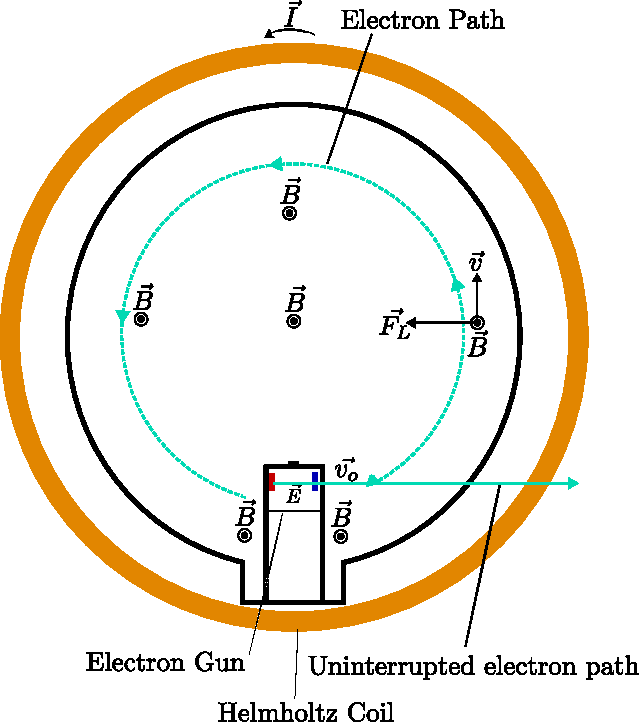
\includegraphics[width=.8\linewidth]{exp02_HelmholtzDiagramV1.pdf}
    \caption{Diagram of the Uchida TG-13 experimental apparatus, with the key components for the experiment, and the uninterrupted and actual electron path noted. In addition the vector directions of key quantities are also present on the diagram}
    \label{fig:diagram}
\end{figure}

Experimentation was performed for different electron gun voltage, and at each voltage multiple currents were used, and the resulting radii recorded. The plot shown below in \ref{fig:vOverB} is the average observed radius   over the ratio of the square root of voltage over the magnetic field strength, the linear regression least squares fit, and the propagated error to the fit of the least squares fit intercepting at the weighted mean of the data set. 

\begin{figure}
    \centering
    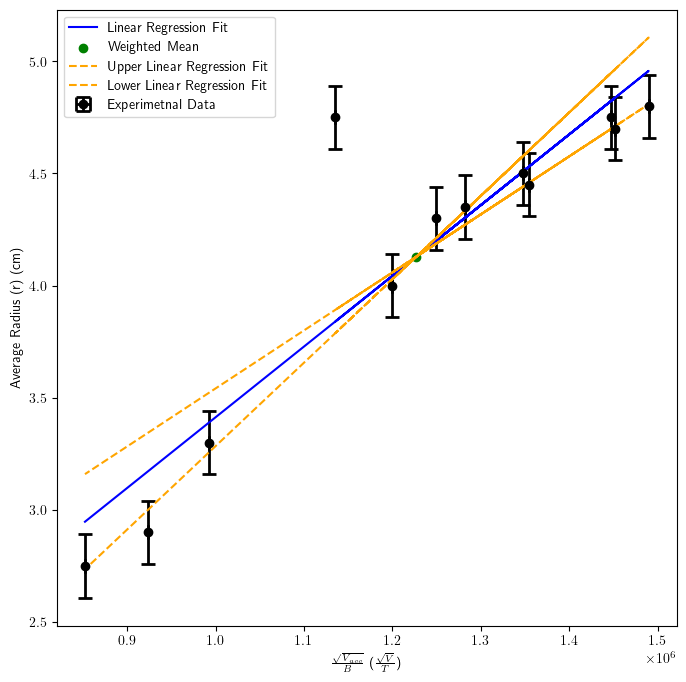
\includegraphics[width=1\linewidth]{sqrtVOverBPlot_V1.png}
    \caption{r vs $\frac{\sqrt{V}}{B}$ plot with the least linear regression best fit line and the associated error to the slope based on the propagation of error from the initial measurements. The slope of the least squares fit line is $m= 3.16 \times10^{-6}\pm9.86\times10^{-7}$ $\frac{\text{cm}}{\frac{\sqrt{\text{\unit{\volt}}}}{T}}$ and a portrayed intercept of $b = .257$, however as seen in the supporting documentation \cite{supp} the intercept is taken to be 0 for its physical meaning and ignored otherwise. }
    \label{fig:vOverB}
\end{figure}

\begin{table}
\begin{tabular}{llll}
$V_acc$ (V) & $I$(mA) & Left Radius (cm) & Right Radius (cm) \\ \hline
\hline 219 & 13.1 & 4.6 $\pm$ .5 & 4.9 $\pm$ .2 \\
219 & 16.7 & 4.6  $\pm$ .5 & 3.7 $\pm$ .2 \\
219 & 14.0 & 4.5 $\pm$ .5 & 4.4 $\pm$ .2 \\
259 & 15.3 & 4.6 $\pm$ .5 & 4.4 $\pm$ .2 \\
259 & 17.2 & 4.1 $\pm$ .5 & 3.9 $\pm$ .2 \\
281 & 14.8 & 4.7 $\pm$ .5 & 4.7 $\pm$ .2 \\
281 & 17.2 & 4.4 $\pm$ .5 & 4.2 $\pm$ .2 \\
296 & 14.8 & 4.7 $\pm$ .5 & 4.9 $\pm$ .2 \\
296 & 17.2 & 4.4 $\pm$ .5 & 4.3 $\pm$ .2 \\
296 & 22.2 & 3.4 $\pm$ .5 & 3.2 $\pm$ .2 \\
256 & 22.2 & 2.9 $\pm$ .5 & 2.9 $\pm$ .2 \\
224 & 22.5 & 2.8 $\pm$ .5 & 2.7 $\pm$ .2 \\ \hline \hline
\end{tabular}
\caption{Compiled experimental data consisting of: electron gun voltage, Helmholtz Coil current, and observed radius at two points, left and right with uncertainty}
\end{table}

From these measurements, data analysis was performed \cite{supp} by using the relation in \eqref{linRBV} with the linear regression line of best fit that was produced. Using this relation it could be found that the slope of the best fit line was equivalent to $\sqrt{\frac{m_e}{q_e}}$. Using this relation, combined with propagating the error through the slope and onto the final value. The magnitude for this value for this quantity was found to be $\text{Ratio} = ( 1.004 \pm .2509 )\times 10^{11}$ \SI{}{C/kg}. Based on more precise measurements taken by NIST, an accepted value for this quantity is taken to be $\text{NIST Value} = 1.758 \times 10^{11}$  $\pm$ $3.1 \times 10^{-10}$  \SI{}{C/kg}. This places the experimentally found value to be within 57$\%$ of the NIST value. While the relative uncertainty of the measured value is 43.6$\%$, this suggests that the calculated value was somewhat close to the reference value. The remaining difference could suggest some form of systemic error to the experiment, such as defects in the equipment used or interference from the environment affecting the path of the electrons.



\section{Conclusions}
In summary, the use of electric and magnetic fields, can be used to guide and control electrons. In this case, electrons were accelerated from an electron gun by a constant voltage ($V_{acc}$) in a low pressure environment. Once accelerated, they were subject to a constant magnetic field orthogonal to their path of travel, produced by a Helmholtz Coil with magnetic field strength (B) running through it. This magnetic field caused the electrons to orbit around a center point in centripetal motion, which provided a measurable radius, from which, the ratio of charge to mass was found. That ratio was found to be $\text{Ratio} = ( 1.004 \pm .2509 )\times 10^{11}$ \SI{}{C/kg}. Within a serviceable range to the reference value of $\text{NIST Value} = 1.758 \times 10^{11}$  $\pm$ $3.1 \times 10^{-10}$  \SI{}{C/kg}. This ratio was determined by fitting a least linear squares regression to the collected data as graphed in Fig. \ref{fig:vOverB} and using \eqref{linRBV}. Future experiments making the same measurement would benefit from several improvements to improve the accuracy of the data. One major improvement would be a more precise way to measure the radius of the electron path, the current method is prone to bias based on the measurer. A better method would be to use some reference to track the path of the electron, such as a checkerboard and see where it intercepts instead of attempting to align a reflection, this could allow for more reproducible and consistent results. Finally, a way to reduce error in the system is increasing the number of points at which each circle is measured, since with more measurements the average uncertainty falls to a point.

\section*{Acknowledgments}
The author would like to acknowledge Brookelyn Velmont for her assistance with the data collection involved for this experiment. 

\section*{Data Availability Statement}
A Jupyter notebook containing all the experimental data, data analysis, figure generation, and additional information on uncertainty analysis can be found in the supplemental materials. \footnote{See online article posting for access to supplemental material.}
\bibliography{biblo}
\end{document}

